

\section{Experimental Results}

In this subsection, we analyze the result quality considering the $C_{max}$ values obtained from the DE algorithm to solve FJSSP, described in previous sections. First, the influence of $Cr$ and $F$ parameters in the DE performance to solve FJSSP is studied (Section~\ref{subsec:Parameters}). Next, the incorporation of the local search process to the DE using different $p_{LS}$ values is analyzed in Section~\ref{subsec:resparallelDELS}. Finally, the parallel implementation of $DE_{LS}$ is considered in Section~\ref{subsec:resparallelDELS}. 

\subsection{Influence of DE Parameters} \label{subsec:Parameters}

The first analysis focuses on the effect of using different combinations of $F$ and $Cr$ values on the performance of DE to solve FJSSP. In particular, both parameters take values in \{0.1, 0.5, 0.9\}, from low to high values. For this purpose, we analyze the result quality taking into account the best $C_{max}$ values obtained for the simple DE algorithm when solving FJSSP instances, and also the number of evaluations needed to reach their best values.

Table~\ref{tab:resultDE} shows the best $C_{max}$ values obtained for the DE algorithm using the different combinations of $F$ and $Cr$ values for each FJSSP instance. Column 2 presents the best-known value of $C_{max}$ (optimal) for each instance. The last row displays the ratio of the number of instances that an algorithm can find its optimum to the total number of instances. 

The DE finds the optimum in 3 instances (MK01, MK03, and MK08) independently from the combinations of $F$ and $Cr$ values considered. The highest value of $F$ offers the less chance of finding the best solutions for the DE regardless of the $Cr$ value used. This combination presents the lowest number of optimal values for the different instances (no more than 4 of the 10 instances). The DE algorithm with the combination of $F=0.5$ and $Cr=0.9$ finds more times the optimal $C_{max}$ value than the others (in 6 of the 10 instances).

An important metric is the relative error or gap of the different best $C_{max}$ values obtained for each DE regarding the optimum of each instance. This metric allows us to normalized the data of the different instances and, in this way, we focus the attention on how different combinations of $F$ and $Cr$ values affect the performance of the DE to solve FJSSP. On the one hand, KW statistical test indicates that there are significant statistical differences between the DE combinations (\textit{p}-value$=2.2e-16$ is lower to the significance level $\alpha = 0.01$). On the other hand, the gap distribution for each combination (see Figure~\ref{fig:DEboxplot}) suggests that the DE algorithm with $F=0.5$ and $Cr=0.9$ presents the lowest median relative error, and also, its box is comparatively short suggesting that overall gap values have a high level of similarity with each other. These observations indicate a superiority of the combination over the other possible ones.  

\begin{figure}[!tb]
    \centering
    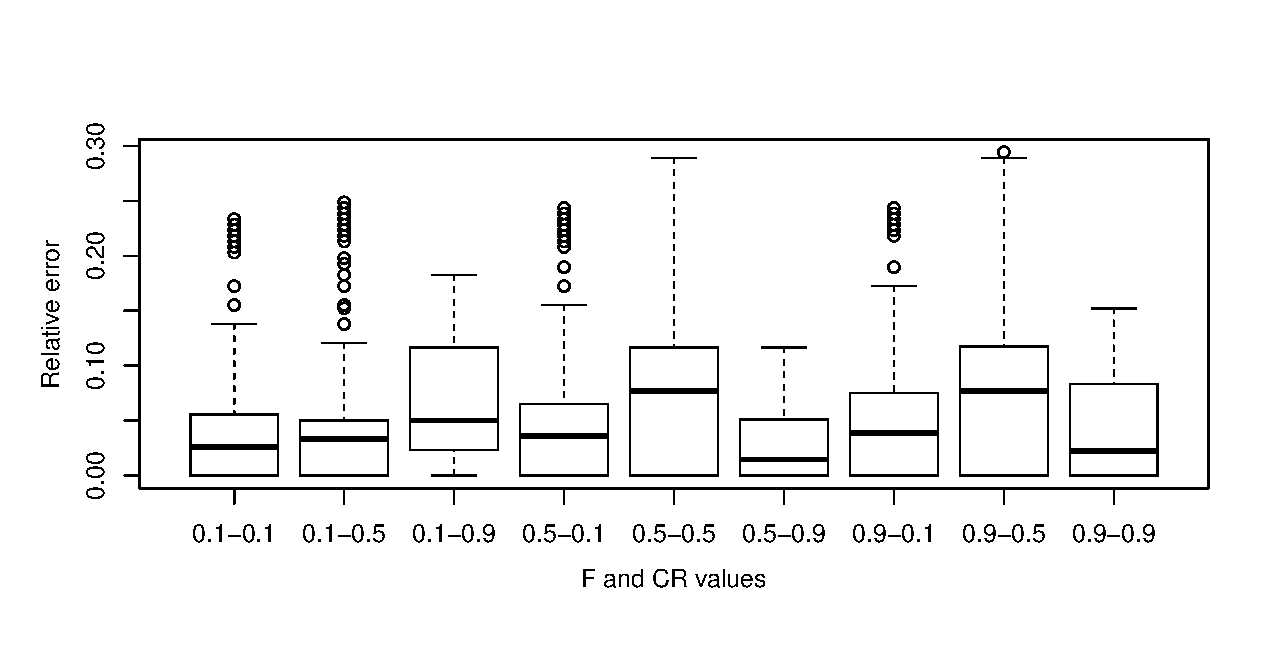
\includegraphics[width=\linewidth]{./figures/Boxplot-DE.eps}
    \caption{Relative error of the DE algorithm for different combinations of $F$ and $Cr$ values.}
    \label{fig:DEboxplot}
\end{figure}
%
\begin{figure*}[htb]
    \centering
    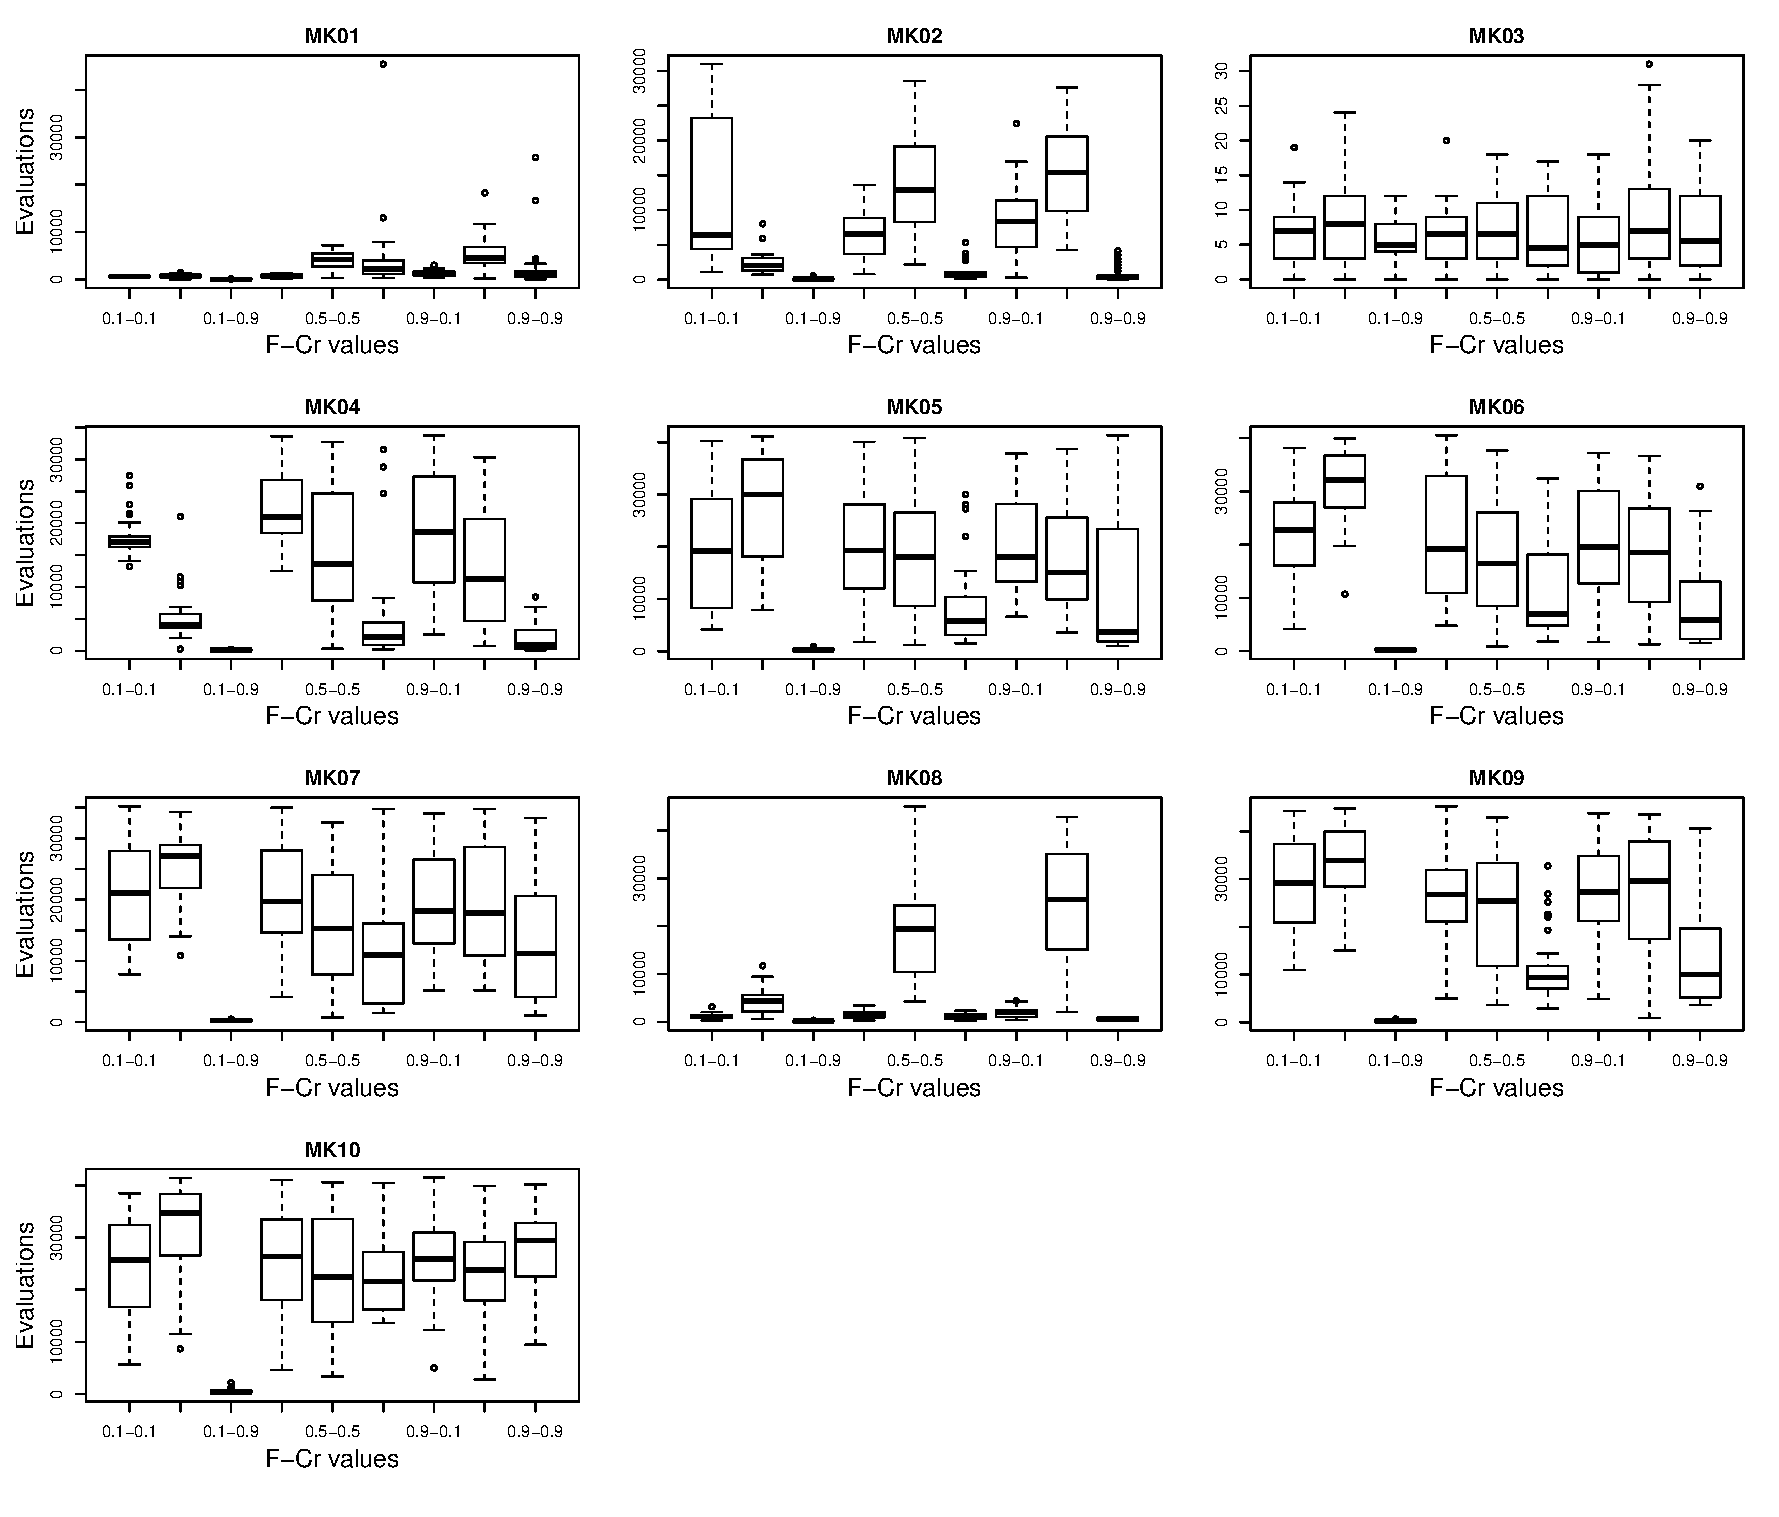
\includegraphics[width=\textwidth]{./figures/DE-evalBest.eps}
    \caption{Number of evaluations to find the best $C_{max}$ value of the DE for different combinations of $F$ and $Cr$ values considering all FJSSP instances.}
    \label{fig:DEevaluations}
    \vspace{-0.4cm}
\end{figure*}

Finally, we proceed to study the distribution of the number of evaluations to find the best $C_{max}$ value performed by DE with different combinations of different $F$ and $Cr$ values. For that purpose, Figure \ref{fig:DEevaluations} illustrates these results employing ten box plot graphs (one for each instance). In general, we observe that the DE algorithm with fewer evaluations is the one with $F\in \{0.1,0.5\}$ and $Cr=0.9$, but the combination $F=0.5$ and $Cr=0.9$ outperforms the other ones from the result quality point of view (see Table~\ref{tab:resultDE}). Consequently, we will adopt $F=0.5$ and $Cr=0.9$ as the parameter settings for the DE in the following experimentation. 

% Table generated by Excel2LaTeX from sheet 'Hoja1'
\begin{table*}[!tb]
  \centering
     \scriptsize
    \label{tab:DELS}
    \caption{Best and mean$_{\pm sd}$ $C_{max}$ values found by the DE$_{LS}$ with different values of $p_{LS}$ for all FJSSP instances.}
    \begin{tabular}{|rrcccrrr|}
    \hline
    \multicolumn{1}{|c}{} & \multicolumn{1}{|c|}{} & \multicolumn{3}{c|}{Best $C_{max}$} & \multicolumn{3}{c|}{Mean$_{\pm sd}$ $C_{max}$} \bigstrut \\
    \cline{3-8}
    \multicolumn{1}{|c|}{\textbf{Inst.}} & \multicolumn{1}{c|}{\textbf{Opt}} & \multicolumn{1}{c|}{\textbf{$p_{LS}=0.1$}} & \multicolumn{1}{c|}{\textbf{$p_{LS}=0.5$}} & \multicolumn{1}{c|}{\textbf{$p_{LS}=0.7$}} & \multicolumn{1}{c|}{\textbf{$p_{LS}=0.1$}} & \multicolumn{1}{c|}{\textbf{$p_{LS}=0.5$}} & \multicolumn{1}{c|}{\textbf{$p_{LS}=0.7$}} \bigstrut\\
    \hline
    \multicolumn{1}{|c|}{Mk01} & \multicolumn{1}{c|}{40} & \multicolumn{1}{c|}{\textbf{40}} & \multicolumn{1}{c|}{\textbf{40}} & \multicolumn{1}{c|}{\textbf{40}} & \multicolumn{1}{c|}{40.00$_{\pm 0.00}$} & \multicolumn{1}{c|}{40.00$_{\pm 0.00}$} & 40.00$_{\pm 0.00}$ \bigstrut\\
    %\hline
    \multicolumn{1}{|c|}{Mk02} & \multicolumn{1}{c|}{26} & \multicolumn{1}{c|}{27} & \multicolumn{1}{c|}{\textbf{26}} & \multicolumn{1}{c|}{\textbf{26}} & \multicolumn{1}{c|}{27.03$_{\pm 0.18}$} & \multicolumn{1}{c|}{26.96$_{\pm 0.18}$} & 26.76$_{\pm 0.43}$ \bigstrut\\
    %\hline
    \multicolumn{1}{|c|}{Mk03} & \multicolumn{1}{c|}{204} & \multicolumn{1}{c|}{\textbf{204}} & \multicolumn{1}{c|}{\textbf{204}} & \multicolumn{1}{c|}{\textbf{204}} & \multicolumn{1}{c|}{204.00$_{\pm 0.00}$} & \multicolumn{1}{c|}{204.00$_{\pm 0.00}$} & 204.00$_{\pm 0.00}$ \bigstrut\\
    %\hline
    \multicolumn{1}{|c|}{Mk04} & \multicolumn{1}{c|}{60} & \multicolumn{1}{c|}{\textbf{60}} & \multicolumn{1}{c|}{\textbf{60}} & \multicolumn{1}{c|}{\textbf{60}} & \multicolumn{1}{c|}{62.00$_{\pm 1.31}$} & \multicolumn{1}{c|}{61.30$_{\pm 0.70}$} & 61.03$_{\pm 0.66}$ \bigstrut\\
    %\hline
    \multicolumn{1}{|c|}{Mk05} & \multicolumn{1}{c|}{172} & \multicolumn{1}{c|}{173} & \multicolumn{1}{c|}{173} & \multicolumn{1}{c|}{173} & \multicolumn{1}{c|}{174.30$_{\pm 0.75}$} & \multicolumn{1}{c|}{173.00$_{\pm 0.00}$ }& 173.00$_{\pm 0.00}$ \bigstrut\\
    %\hline
    \multicolumn{1}{|c|}{Mk06} & \multicolumn{1}{c|}{58} & \multicolumn{1}{c|}{63} & \multicolumn{1}{c|}{62} & \multicolumn{1}{c|}{61} & \multicolumn{1}{c|}{64.40$_{\pm 0.56}$} & \multicolumn{1}{c|}{62.83$_{\pm 0.53}$} & 62.43$_{\pm 0.62}$ \bigstrut\\
    %\hline
    \multicolumn{1}{|c|}{Mk07} & \multicolumn{1}{c|}{139} & \multicolumn{1}{c|}{142} & \multicolumn{1}{c|}{140} & \multicolumn{1}{c|}{140} & \multicolumn{1}{c|}{143.20$_{\pm 0.69}$} & \multicolumn{1}{c|}{142.00$_{\pm 0.90}$} & 141.80$_{\pm 0.92}$ \bigstrut\\
    %\hline
    \multicolumn{1}{|c|}{Mk08} & \multicolumn{1}{c|}{523} & \multicolumn{1}{c|}{\textbf{523}} & \multicolumn{1}{c|}{\textbf{523}} & \multicolumn{1}{c|}{\textbf{523}} & \multicolumn{1}{c|}{523.00$_{\pm 0.00}$} & \multicolumn{1}{c|}{523.00$_{\pm 0.00}$} & 523.00$_{\pm 0.00}$ \bigstrut\\
    %\hline
    \multicolumn{1}{|c|}{Mk09} & \multicolumn{1}{c|}{307} & \multicolumn{1}{c|}{309} & \multicolumn{1}{c|}{\textbf{307}} & \multicolumn{1}{c|}{\textbf{307}} & \multicolumn{1}{c|}{313.10$_{\pm 2.20}$} & \multicolumn{1}{c|}{310.00$_{\pm 1.33}$} & 309.00$_{\pm 1.72}$ \bigstrut\\
    %\hline
    \multicolumn{1}{|c|}{Mk10} & \multicolumn{1}{c|}{197} & \multicolumn{1}{c|}{226} & \multicolumn{1}{c|}{225} & \multicolumn{1}{c|}{224} & \multicolumn{1}{c|}{231.10$_{\pm 2.41}$} & \multicolumn{1}{c|}{228.00$_{\pm 1.36}$} & 227.20$_{\pm 1.38}$ \bigstrut\\
    \hline
    \multicolumn{2}{c|}{}   & 4/10  & 6/10  &\multicolumn{1}{c|}{6/10}\bigstrut\\
    \cline{3-5}
    \end{tabular}%
  \label{tab:DELS}%
\end{table*}%

\subsection{Results of the DE with Local Search} \label{subsec:resDELS}

The following analysis goes into detail of what happened when the DE algorithm is enhanced with a local search procedure to solve FJSSP. The resulting algorithm is named DE$_{LS}$. For this study, we consider three different $p_{LS}$ values in the set \{0.1, 0.5, 0.7\}, i.e. we study how the frequency of the LS impacts the DE performance by using low, medium, and high probability values.

Table~\ref{tab:DELS} shows the best and the mean $C_{max}$ values, together the standard deviation, found by the DE$_{LS}$ with the different $p_{LS}$ values. The DE$_{LS}$ obtains more times the optimum when $p_{LS}=0.5$ or $p_{LS}=0.7 $.  Moreover, the KW test indicates that there are statistically significant differences among the algorithms ($p$-values are lower than the level of significance). The DE$_{LS}$ using the highest frequency ($p_{LS}=0.7$) has the lowest mean $C_{max}$ values for all instances, suggesting that the algorithm can find the optimum or near-optimal $C_{max}$ values in the majority of the runs. This assumption is reflected in the boxplot of the relative error presented in Figure \ref{fig:DELSboxplot}, which shows that the median error value is lower with the highest local search frequency.
%
\begin{figure}[!tb]
    \centering
    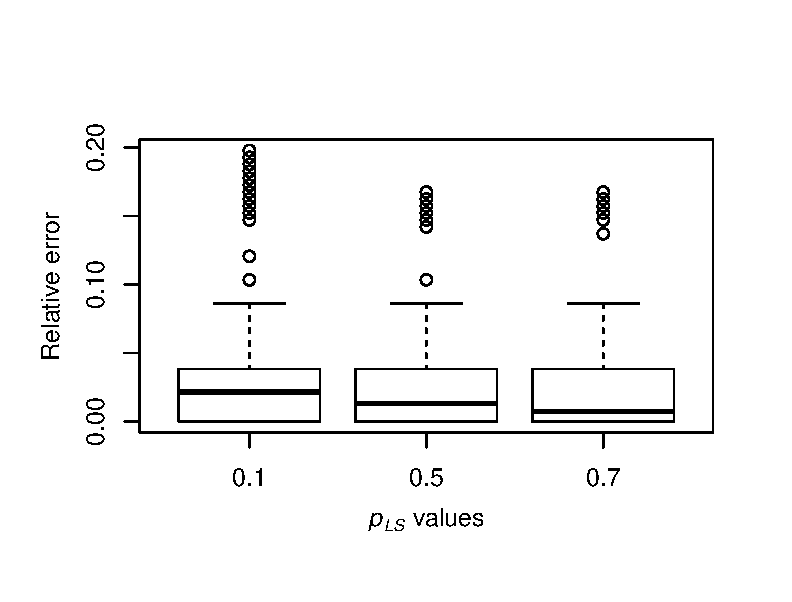
\includegraphics[width=\linewidth]{./figures/Boxplot-DELS.eps}
    \caption{Relative error of the DE$_{LS}$  for different values of $p_{LS}$.}
    \label{fig:DELSboxplot}
\end{figure}
%
\begin{figure}[!tb]
\scriptsize
\centering
   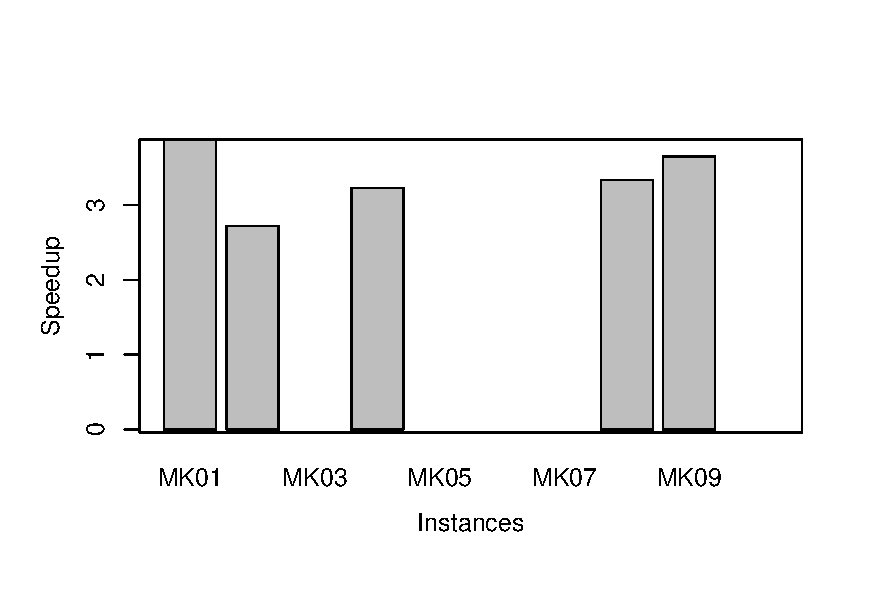
\includegraphics[width=\linewidth]{figures/speedup.eps}
   \vspace{-0.9cm}
    \caption{Speedup by FJSSP instances.}
    \label{fig:speedup}
\end{figure}
%
\begin{table*}[!tb]
\scriptsize
  \centering
  \caption{Comparison between DE$_{LS}$ and population-based metaheuristics from the literature}
    \begin{tabular}{|l|cccccccccc|}
    \hline
    \multicolumn{1}{|r}{} & \multicolumn{1}{l}{MK01} & \multicolumn{1}{l}{MK02} & \multicolumn{1}{l}{MK03} & \multicolumn{1}{l}{MK04} & \multicolumn{1}{l}{MK05} & \multicolumn{1}{l}{MK06} & \multicolumn{1}{l}{MK07} & \multicolumn{1}{l}{MK08} & \multicolumn{1}{l}{MK09} & \multicolumn{1}{l|}{MK10} \\
    \hline
    DE$_{LS}$   & \textbf{40} & \textbf{26} & \textbf{204} & \textbf{60} & 173   & 61    & 140   & \textbf{523} & \textbf{307} & 224 \\
    hGA   & \textbf{40} & \textbf{26} & \textbf{204} & 62    & \textbf{172} & 65    & 140   & \textbf{523} & 310   & 214 \\
    BEDA  & \textbf{40} & \textbf{26} & \textbf{204} & \textbf{60} & \textbf{172} & 60    & \textbf{139} & \textbf{523} & \textbf{307} & 206 \\
    IACO  & \textbf{40} & \textbf{26} & \textbf{204} & \textbf{60} & 173   & 60    & 140   & \textbf{523} & \textbf{307} & 208 \\
    HDE   & \textbf{40} & \textbf{26} & \textbf{204} & \textbf{60} & \textbf{172} & \textbf{57} & \textbf{139} & \textbf{523} & \textbf{307} & \textbf{198} \\
\hline
    \end{tabular}%
  \label{tab:comparison}%
\end{table*}%
%
Now, to determine if the DE$_{LS}$ can improve the $C_{max}$ values found by the DE, we perform a comparison of relative error values shown in Figure~\ref{fig:DEboxplot} and the ones from Figure~\ref{fig:DELSboxplot}. We can observe that the DE$_{LS}$ algorithm with $p_{LS}=0.7$ obtains lower relative errors than those presented by DE, which indicates the advantage of incorporating local search into the DE framework.

\subsection{Results of the DE$_{LS}$ and Parallelism} \label{subsec:resparallelDELS}

In this section, we study the behavior of the parallel DE described in Section~\ref{subsec:parallelHDE}. The most important measure of a parallel algorithm is speedup. This measure is defined as the ratio of the sequential execution time (DE$_{LS}$ execution time, in this case) to the parallel execution time. For this analysis, we consider the weak speedup~\cite{albaMeta2005}. For that reason and following the best practice by Luque and Alba~\cite{Luque:2013:PGA:2564896}, the stopping criterion is based on the quality of the final solution achieved by the algorithms, which is set to the optimum for each FJSSP instance (see column Opt. of Table~\ref{tab:resultDE}). Consequently, the speedup values are only reported for those instances for which the DE$_{LS}$ algorithm obtains the optimum value.

Once we established the execution times of the DE$_{LS}$ and the parallel DE$_{LS}$, we calculate the speedup values. Figure~\ref{fig:speedup} shows that the use of parallelization is worthwhile, as we expected. The parallel DE$_{LS}$ allows to reduce the search time and obtains a very good speed up, nearby linear (the ideal speedup value is 4, the number of available cores per machine).

\section{Comparison of DE$_{LS}$ with the Literature} \label{sec:compara}

Finally, we present a comparative assessment of the $C_{max}$ values obtained by the DE$_{LS}$ with the ones of several competitive algorithms present in the literature to solve FJSSP. This allows us to determine the goodness of the metaheuristics considered in this work. In this comparison different population-based metaheuristics to solve FJSSP are considered: 
\begin{enumerate}[label=\textit{\roman*})]

\item hGA~\cite{tang2011}: a hybrid algorithm combining chaos particle swarm optimization with genetic algorithm

\item BEDA~\cite{Wang2012917}: a bi-population based estimation of distribution algorithm

\item IACO~\cite{WANG2017}: an ant colony optimization

\item HDE~\cite{YUAN2013246}: a hybrid differential evolutionary algorithm 

\end{enumerate}

Table~\ref{tab:comparison} shows that the $C_{max}$ values obtained by DE$_{LS}$ are similar to the ones of remaining algorithms, for the majority of the ten instances. This observation suggests that the DE$_{LS}$ proposed in this work is a competitive algorithm to solve FJSSP. Comparisons regarding computational effort are hard to be carried out because the majority of the works do not report the number of evaluations. Consequently, the relative efficiency of referred algorithms is difficult to contrast to obtain meaningful comparisons.


